\documentclass{article}

\usepackage{graphicx}
\usepackage{tikz}
\usepackage{tikzsymbols}
\usetikzlibrary{calc,patterns,shapes.geometric}
\pagestyle{empty}
\usepackage[margin=0pt]{geometry}
\geometry{papersize={14in,12in}}

\def\centerarc[#1](#2)(#3:#4:#5){\draw[#1] ($(#2)+({#5*cos(#3)},{#5*sin(#3)})$) arc (#3:#4:#5);}

\begin{document}
	\begin{figure}
		\centering
		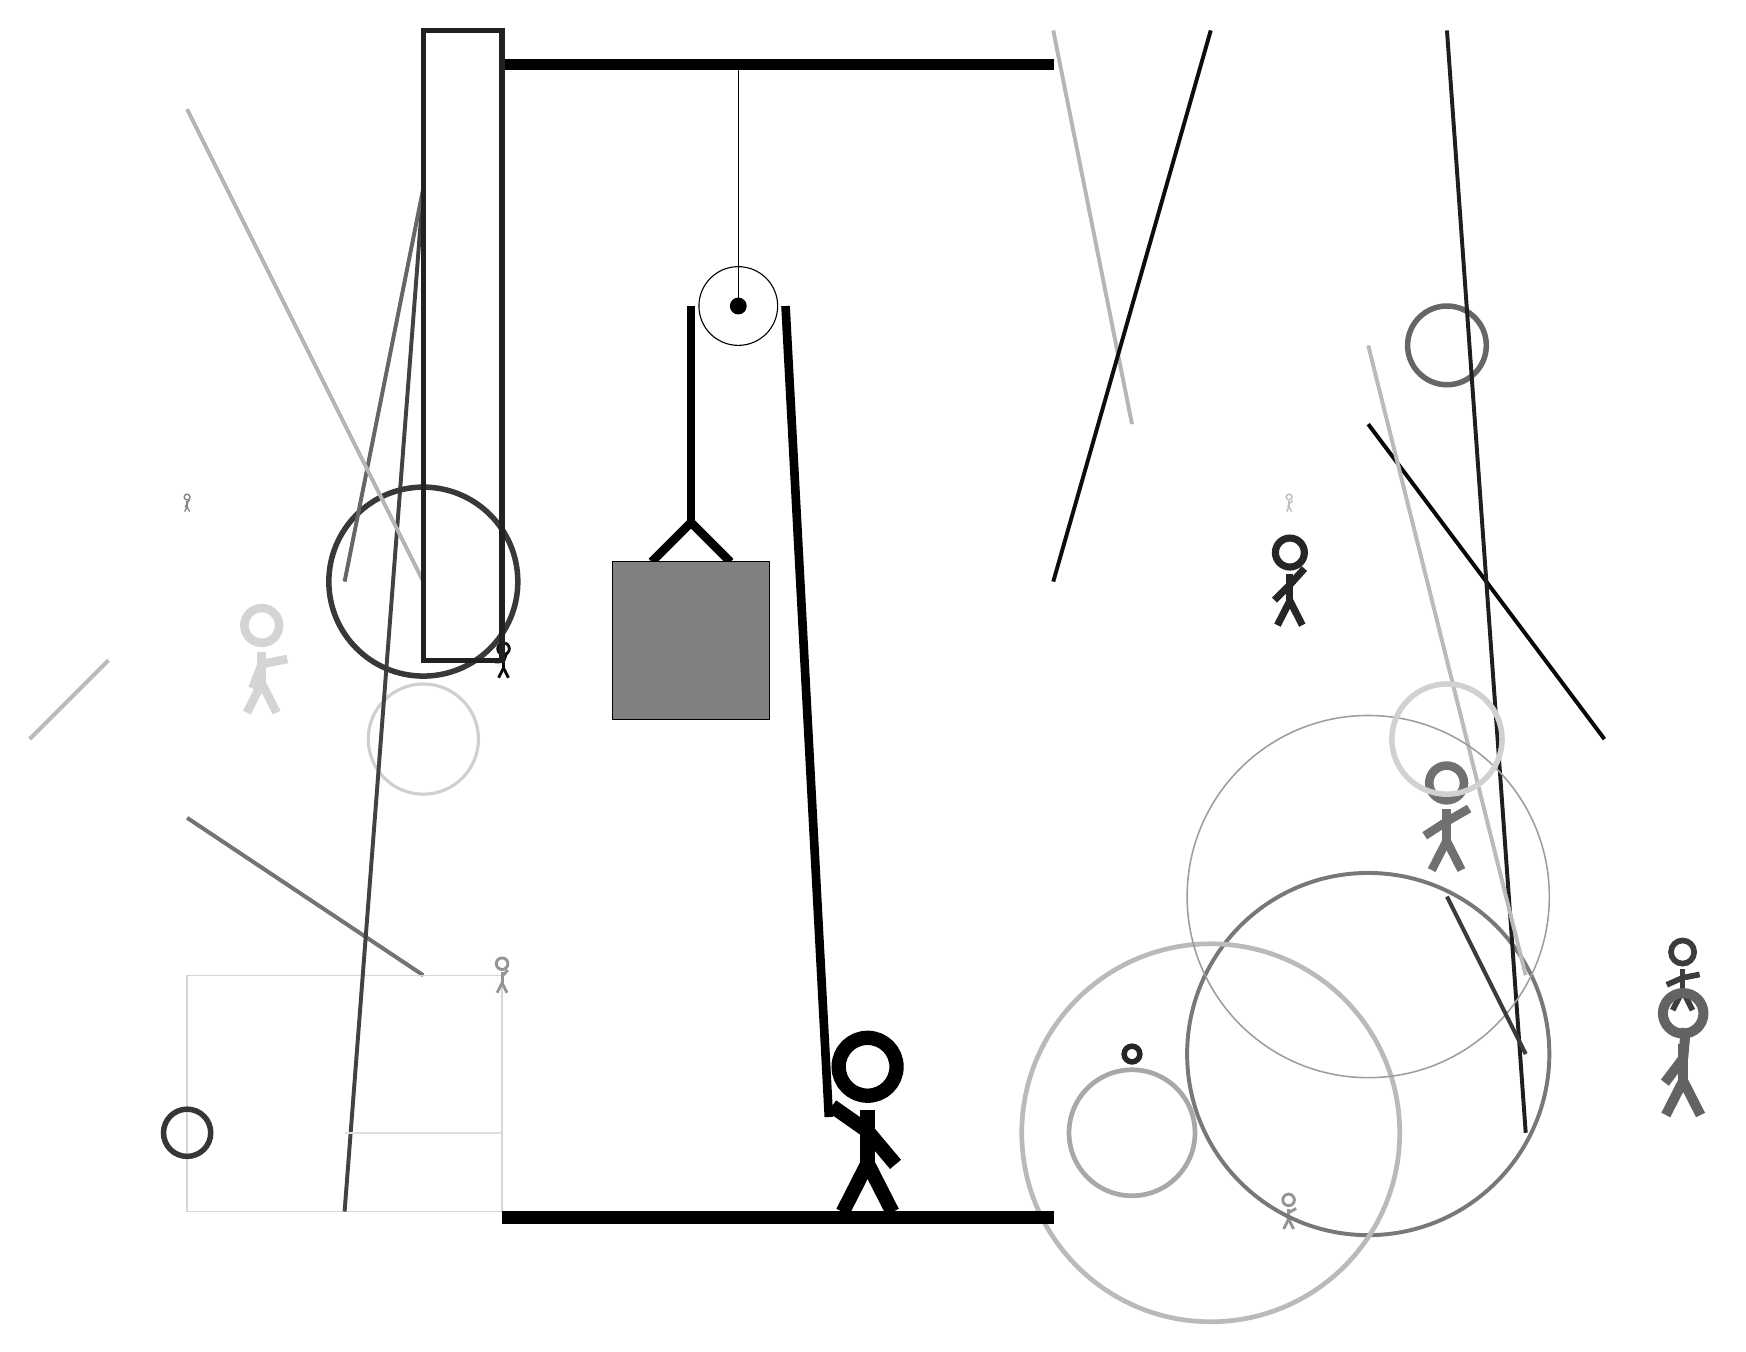
\begin{tikzpicture}
			%%%%% START %%%%%
			
			\draw[fill=black] (-2, 11.5) rectangle (5, 11.625);
			
			\draw (1, 8.5) circle (0.5);
			\draw[fill=black] (1, 8.5) circle (0.1);
			\draw (1, 11.5) -- (1, 8.5);
			
			\draw [line width=0.6mm, color=black!34](6, -2) circle (0.8);
			
			\draw[line width=0.5mm, color=black!55](-6, 2) -- (-3, 0);
			\draw[line width=0.2mm, color=black!16] (-2, -3) rectangle (-6, 0);
			\draw [line width=0.4mm, color=black!19](-3, 3) circle (0.7);
			
			\node[line width=0.5mm, color=black!95] at (-2, 4) {\Strichmaxerl[2][3][70]};
			\draw [line width=0.7mm, color=black!60](10, 8) circle (0.5);
			\node[line width=0.2mm, color=black!42] at (-2, 0) {\Strichmaxerl[2][90][49]};
			\draw[line width=0.5mm, color=black!29](6, 7) -- (5, 12);
			\node[line width=0.5mm, color=black!42] at (8, -3) {\Strichmaxerl[2][84][30]};
			
			\node[line width=0.2mm, color=black!25] at (8, 6) {\Strichmaxerl[1][71][35]};
			\draw[line width=0.5mm, color=black!74](-4, -3) -- (-3, 10);
			\draw [line width=0.5mm, color=black!53](9, -1) circle (2.3);
			\draw [line width=0.7mm, color=black!60](-2, 0) circle (0.0);
			
			\draw[line width=0.6mm, color=black!62] (-2, 3) rectangle (-2, 3);
			\node[line width=0.3mm, color=black!56] at (10, 2) {\Strichmaxerl[6][33][30]};
			\draw [line width=0.7mm, color=black!78](-3, 5) circle (1.2);
			
			\node[line width=0.6mm, color=black!47] at (-6, 6) {\Strichmaxerl[1][64][59]};
			
			\node[line width=0.7mm, color=black!85] at (8, 5) {\Strichmaxerl[5][45][48]};
			\draw [line width=0.7mm, color=black!85](6, -1) circle (0.1);
			\node[line width=0.7mm, color=black!76] at (13, 0) {\Strichmaxerl[4][24][11]};
			\draw[line width=0.5mm, color=black!97](9, 7) -- (12, 3);
			\draw[line width=0.5mm, color=black!88](10, 12) -- (11, -2);
			\draw[line width=0.5mm, color=black!27](-7, 4) -- (-8, 3);
			\draw [line width=0.6mm, color=black!27](7, -2) circle (2.4);
			\draw[line width=0.3mm, color=black!13] (-2, -2) rectangle (-4, -2);
			
			\draw[line width=0.5mm, color=black!60](-4, 5) -- (-3, 10);
			
			\draw[line width=0.5mm, color=black!95](5, 5) -- (7, 12);
			\draw [line width=0.7mm, color=black!79](-6, -2) circle (0.3);
			\node[line width=0.4mm, color=black!17] at (-5, 4) {\Strichmaxerl[6][69][11]};
			
			\draw[line width=0.5mm, color=black!27](9, 8) -- (11, 0);
			\draw [line width=0.2mm, color=black!38](9, 1) circle (2.3);
			
			\draw[line width=0.5mm, color=black!29](-6, 11) -- (-3, 5);
			\draw[line width=0.5mm, color=black!77](10, 1) -- (11, -1);
			\draw [line width=0.7mm, color=black!18](10, 3) circle (0.7);
			
			\node[line width=0.3mm, color=black!61] at (13, -1) {\Strichmaxerl[7][53][85]};
			\draw[line width=0.7mm, color=black!87] (-3, 12) rectangle (-2, 4);
			
			\draw[line width=1.1mm] (-0.1, 5.25) -- (0.4, 5.75) -- (0.9, 5.25);
			\draw[fill=black!50] (-0.6, 5.25) rectangle (1.4, 3.25);
			
			\draw[line width=1.1mm] (0.4, 8.5) -- (0.4, 5.75);
			\centerarc[line width=1.1mm](1, 8.5)(0:180:0.6);
			\draw[line width=1.1mm](1.6, 8.5) -- (2.15, -1.8);
			
			\node at (2.6, -1.9) {\Strichmaxerl[10][-35][-50]};
			
			\draw[fill=black] (-2, -3) rectangle (5, -3.15);
			
			%%%%% END %%%%%
		\end{tikzpicture}
	\end{figure}	
\end{document}